%%%%%%%%%%%%%%%%%%%%%%%%%%%%%%%%%%%%%%%%%%%%%%%%%%%%%%%%%%%%%%%%%%%%%%%%%%%%%%%%
%2345678901234567890123456789012345678901234567890123456789012345678901234567890
%        1         2         3         4         5         6         7         8

\documentclass[letterpaper, 10 pt, conference]{ieeeconf}  % Comment this line out
                                                          % if you need a4paper
%\documentclass[a4paper, 10pt, conference]{ieeeconf}      % Use this line for a4
                                                          % paper

\IEEEoverridecommandlockouts                              % This command is only
                                                          % needed if you want to
                                                          % use the \thanks command
\overrideIEEEmargins
% See the \addtolength command later in the file to balance the column lengths
% on the last page of the document

\usepackage[utf8]{inputenc}
\usepackage[T1]{fontenc}
\usepackage{hyperref}
\usepackage{xcolor}

\definecolor{navy}{RGB}{0, 0, 128}

% The following packages can be found on http:\\www.ctan.org
\usepackage{graphicx} % for pdf, bitmapped graphics files
%\usepackage{epsfig} % for postscript graphics files
%\usepackage{mathptmx} % assumes new font selection scheme installed
%\usepackage{mathptmx} % assumes new font selection scheme installed
%\usepackage{amsmath} % assumes amsmath package installed
%\usepackage{amssymb}  % assumes amsmath package installed

\title{\LARGE \bf
Comparing RSSI Between Thinly Enclosed and Exposed Devices 
}

%\author{ \parbox{3 in}{\centering Huibert Kwakernaak*
%         \thanks{*Use the $\backslash$thanks command to put information here}\\
%         Faculty of Electrical Engineering, Mathematics and Computer Science\\
%         University of Twente\\
%         7500 AE Enschede, The Netherlands\\
%         {\tt\small h.kwakernaak@autsubmit.com}}
%         \hspace*{ 0.5 in}
%         \parbox{3 in}{ \centering Pradeep Misra**
%         \thanks{**The footnote marks may be inserted manually}\\
%        Department of Electrical Engineering \\
%         Wright State University\\
%         Dayton, OH 45435, USA\\
%         {\tt\small pmisra@cs.wright.edu}}
%}

\author{Samrat Sahoo, samratsahoo2013@gmail.com}
% <-this % stops a space
\begin{document}


\maketitle
\thispagestyle{empty}
\pagestyle{empty}


%%%%%%%%%%%%%%%%%%%%%%%%%%%%%%%%%%%%%%%%%%%%%%%%%%%%%%%%%%%%%%%%%%%%%%%%%%%%%%%%
\begin{abstract}

In this paper, we explore the idea of automatic contact tracing through bluetooth devices. More specifically, this paper presents an in-depth analysis of the RSSI values between thinly enclosed devices and completely exposed devices at different distances. Then a regression and proximity detection algorithm is presented to synthesize the results of the data collected.
\smallbreak
Keywords—RSSI, Bluetooth, Raspberry Pi, Regression, Log Normal Shadowing Model
\end{abstract}
\begin{Code}
\bf Code \& Data—\color{navy}\href{https://github.com/SamratSahoo/RPi-Contact-Tracer}{https://github.com/SamratSahoo/RPi-Contact-Tracer}
\end{Code}
%%%%%%%%%%%%%%%%%%%%%%%%%%%%%%%%%%%%%%%%%%%%%%%%%%%%%%%%%%%%%%%%%%%%%%%%%%%%%%%%
\section{INTRODUCTION}

\subsection{Project Description}
This project addresses one primary aspect of the PACT project: thin enclosing versus no enclosing. When using bluetooth devices, such as smartphones, majority of the time they will be inside the user's pocket or similar location. For that reason, it is incumbent to compare when the device is covered by a thin enclosing such as the cloth of clothes and when it is completely out in the open. This project attempts to find variations or patterns between the receiving signal strength indicator (RSSI) when the device in a thin enclosing and no enclosing.

\subsection{Background Information}
In this experiment, we utilize the bluetooth features from two Raspberry Pis. One Raspberry Pi acts as the advertiser which sends out signals. These signals are then picked up by the other Raspberry Pi which acts as the scanner. The bluetooth signal strength is measured by its receiving signal strength indicator or RSSI. A stronger RSSI will have values closer to 0 dBm while weaker RSSI will have values closer to -100 dBm which marks the weakest an RSSI can become. In this experiment, we make the following assumptions:
\begin{itemize}
\item The state of the environment will stay constant in a 10x10 meter square area as long as the two devices are not moved outside of it.  
\item Interactions that require bluetooth contact tracing will primarily occur indoors therefore this project was conducted indoors.
\item The recorded RSSI will stay constant if a device is rebooted.
\item The RSSI values recorded from different materials will scale the same depending on the attenuation factor. Therefore, the material used during as the obstruction will not matter for the final data analysis.



\end{itemize}
\section{HYPOTHESIS}
\subsection{Significance to Bluetooth Contact Tracing}
\begin{itemize}
\item This project is incumbent to studying bluetooth signals with different obstructions as this project reveals the relationships between the RSSI values of thinly enclosed and exposed devices.
\item This project presents an alternative form of the Log Normal Shadowing Model which converts RSSI values into distances.
\item This project allows us to find patterns or relationships between RSSI values in different enclosures.
\end{itemize}
\subsection{Hypothesis and Investigation}

This experiment was designed to check whether or not a relationship exists between RSSI values between a device that is thinly enclosed versus a device that is completely exposed. The hypothesis taken is that there would be weaker RSSI values from the device that was thinly enclosed because obstructions would cause interference.
\smallbreak
In order to test out this hypothesis, the most intensive part of the investigation is the data analysis. With the data analysis, several statistical measures will be needed to be taken in order to cover all relationships between the RSSI values of thinly enclosed and exposed devices.

\section{EXPERIMENTS AND DATA COLLECTIONS}

\subsection{Overview}
In this experiment, there were two main iterations of work: the first iteration tested the RSSI values in an exposed state and the second iteration tested the RSSI values in an thinly enclosed state. This process was repeated at the distances of 0, 2, 4, 6, 8, and 10 meters.

\subsection{Plan and Execution}
Prior to the actual experimentation, one Raspberry Pi was setup with a scanner configuration and the other Raspberry Pi setup with an advertiser configuration. The configurations are as follows in Table I:

\begin{table}[h]
\caption{Scanner Configuration}
\label{table_example}
\begin{center}
\begin{tabular}{|c|c|}
\hline
Timeout & 100 Seconds\\
\hline
Scanning Interval & 1 Second\\
\hline
Filters & None\\
\hline
\end{tabular}
\end{center}
\end{table}

In Table II, the configurations for the advertiser are found:
\begin{table}[h]
\caption{Advertiser Configuration}
\label{table_example}
\begin{center}
\begin{tabular}{|c|c|}
\hline
Timeout & None\\
\hline
Major Value & 1\\
\hline
Minor Value & 1\\
\hline
TX Power & 1\\
\hline
Advertising Interval & 20 ms\\
\hline
\end{tabular}
\end{center}
\end{table}

In order to conduct this experiment, one Raspberry Pi was set as the advertiser and the other as the scanner. The scanner would then run the core program to record RSSI values and put them into a CSV file. This was done for each distance starting from 0 meters and ranging to 10 meters with a 2 meter interval. The scanners would record for 100 seconds before ceasing operations. This whole process would then be repeated except this time with a thin enclosure.
\smallbreak
The primary limitations of this project regarded control over the environment variables and their effect on this experiment. For that reason, the environment was kept constant so that discrepancies between a changing environment would zero out.
\subsection{Data Relevance}
The data that was collected and analyzed consisted of the first 50 scans of the advertiser at 0,2,4,6,8 and 10 meters with one trial being thinly enclosed and the one trial being exposed. This was done so we could properly measure the relationship between the advertiser and scanner not just at one distance but several. This proved helpful when comparing the average RSSI between both states.  
\subsection{Examples}
The raw data that was collected was in the form of RSSI value versus scan number at distances of 0,2,4,6,8, and 10 meters in a thinly enclosed state and exposed state. Sample data for the RSSI values for 0 meters for a thinly enclosed and exposed Raspberry Pi can be found on Table III and Table IV:
\begin{table}[h]
\caption{Scan Number Versus RSSI Value - 0 Meters Thinly Enclosed}
\label{table_example}
\begin{center}
\begin{tabular}{|c|c|}
\hline
\bf Scan Number & \bf RSSI Value (dBm)\\
\hline
1 & -26\\
\hline
2 & -26\\
\hline
3 & -32\\
\hline
4 & -26\\
\hline
\end{tabular}
\end{center}
\end{table}

\begin{table}[h]
\caption{Scan Number Versus RSSI Value - 0 Meters Exposed}
\label{table_example}
\begin{center}
\begin{tabular}{|c|c|}
\hline
\bf Scan Number & \bf RSSI Value (dBm)\\
\hline
1 & -36\\
\hline
2 & -31\\
\hline
3 & -31\\
\hline
4 & -30\\
\hline
\end{tabular}
\end{center}
\end{table}

Graphing the RSSI Values for 0 meters we get the following graph:
   \begin{figure}[thpb]
      \centering
      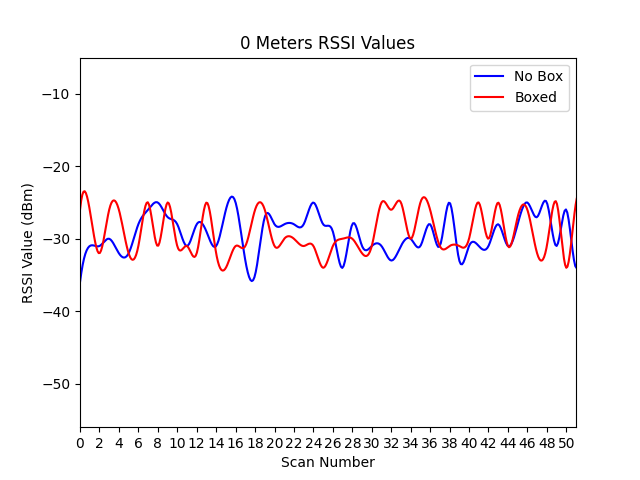
\includegraphics[scale=0.5]{0Meters.png}
      \caption{First 50 scans RSSI Values of a Thinly Exposed (Boxed) and Exposed (No Box) Raspberry Pi at 0 meters of distance}
      \label{figurelabel}
   \end{figure}

Graphs and data for the other distances can be found at the data and code repository.


\section{ANALYSIS AND ALGORITHMS}
\subsection{Statistical Analysis}
\subsubsection{Mean RSSI Values}
The mean RSSI values of each distance for a thinly enclosed and exposed device were graphed in order to note substantial pattern differences between the two states of the device.
   \begin{figure}[thpb]
      \centering
      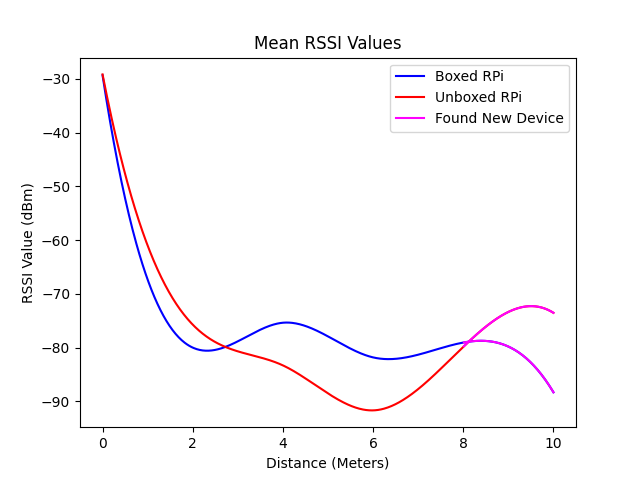
\includegraphics[scale=0.5]{MeanGraph.png}
      \caption{Mean RSSI Values of a thinly enclosed and exposed device from 0 - 10 meters based on collected data}
      \label{figurelabel}
   \end{figure}
\smallbreak
In graphing the mean RSSI values for each distance, we notice that after the 8 meter mark both the thinly enclosed and exposed devices are not found. Additionally, no significant differences in RSSI values or patterns between the thinly enclosed and exposed devices were found because the shape of the graph stayed, relatively speaking, the same. Therefore when comparing the RSSI values at face, there is no significant change between the states.
\subsubsection{Standard Deviation of RSSI Values}
The standard deviation of the RSSI values were graphed in order to study the behavior of the RSSI values at each distance and compare a thinly enclosed device behavior with an exposed device behavior.
   \begin{figure}[thpb]
      \centering
      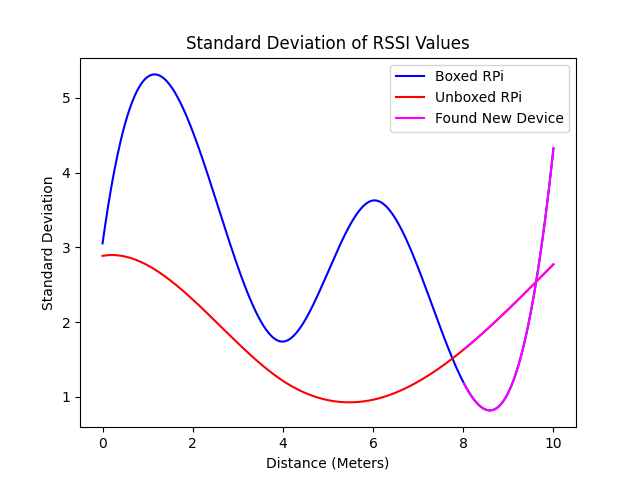
\includegraphics[scale=0.5]{StandardDeviation.png}
      \caption{Standard Deviation of RSSI Values of a thinly enclosed and exposed device from 0 - 10 meters based on collected data}
      \label{figurelabel}
   \end{figure}
\smallbreak
The graph depicts that the standard deviation of the a thinly enclosed Raspberry Pi is significantly higher than the standard deviation for a exposed device. This is likely caused by the blockage from the enclosing which could cause for signals to only sometimes go through or become scattered. However, the exact reason is unknown. 
\subsection{Algorithms}
\subsubsection{Polynomial Regression for Mean RSSI}
In order to generalize the data into a form that could be used for any distance, a polynomial regression was used to form a model that outputted an RSSI based on the distance. The mean RSSI value data was used in order to form this model. Figure 4 depicts the regression:
   \begin{figure}[thpb]
      \centering
      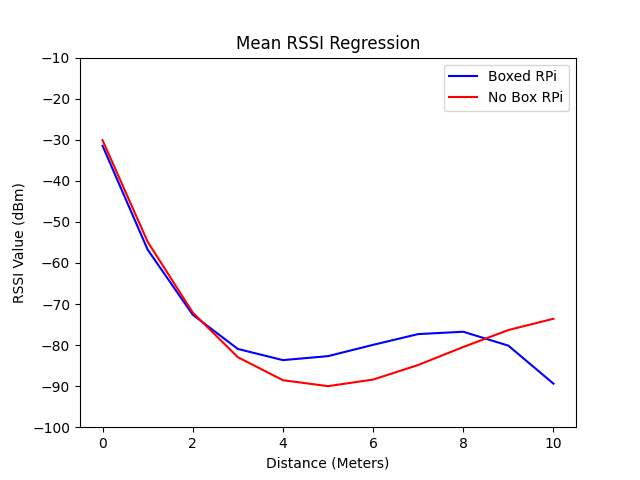
\includegraphics[scale=0.5]{MeanRegression.png}
      \caption{Polynomial Regression of mean RSSI Values of a thinly enclosed and exposed device from 0 - 10 meters}
      \label{figurelabel}
   \end{figure}
\smallbreak
As shown from the regression, both the thinly enclosed and exposed devices had very similar regressions, suggesting that the actual variance in RSSI value between both states was not large and therefore the RSSI strength hardly differed from the thinly enclosed and exposed devices.
\smallbreak
\subsubsection{Modified  Log  Normal  Shadowing  Model}
The log normal shadowing model is used to get estimates of distances based on RSSI values. The regular Log Normal Shadowing Model can be represented as follows:
\begin{equation}
    D = (10^\frac {R - A_0}{-10*n}) + c
\end{equation}
The parts of the Log Normal Shadowing Model are as follows:
\begin{itemize}
\item $D$: Distance 
\item $R$; RSSI Value
\item $A_0$: Average RSSI value at a distance of 1m from the advertiser
\item $n$: This is the signal propagation exponent It is a constant that differs from environment to environment. It ranges from 0 to 5.
\item $c$: This is the environment constant which is used to add weight to reduce the error. It differs from environment to environment.
\end{itemize}
\smallbreak
With RSSI, devices differ from one another so the bluetooth signal from one device will not equate to the same signal for another device. This in turn caused different calculated distances from the same distance using the Log Normal Shadowing Model. Therefore, the Log Normal Shadowing Model does not apply to all devices. 
\smallbreak
To make the the Log Normal Shadowing Model applicable to all devices, a parameter, the device constant, is added. The device constant will differ from device to device and should be tuned manually. From this a modified Log Normal Shadowing Model emerges. $D_C$ is used to represent the device constant. It can be represented as follows:
\begin{equation}
    D = ((10^\frac {R - A_0}{-10*n}) + c) \cdot D_C
\end{equation}
The goal of developing this algorithm was to get an RSSI versus distance relationship that would be applicable to the Raspberry Pis that were used in this experiment. Through repetitive experimentation, applying the following parameters in Table V, Figure 5 is representative of this experiment:
\begin{table}[h]
\caption{Parameters for Modified Log Normal Shadowing Model}
\label{table_example}
\begin{center}
\begin{tabular}{|c|c|}
\hline
\bf Paramter & \bf Value \\
\hline
$A_0$ & -50\\
\hline
$n$ & 5\\
\hline
$c$ & 1\\
\hline
$D_C$ & 0.5\\
\hline
\end{tabular}
\end{center}
\end{table}
   \begin{figure}[thpb]
      \centering
      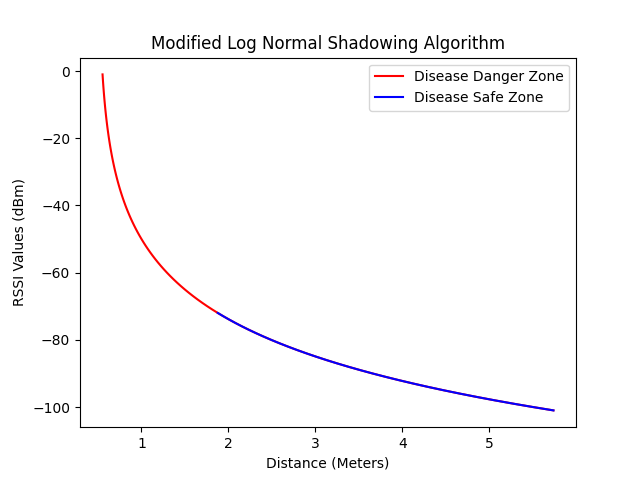
\includegraphics[scale=0.5]{ModelGraph.png}
      \caption{Modified Log Normal Shadowing Graph}
      \label{figurelabel}
   \end{figure}
\smallbreak

\section{CONCLUSIONS}
\subsection{Hypothesis Evaluation}
Originally, it was hypothesized that the RSSI strengths would decrease in a thinly enclosed device because of the obstructions. Through these experiments, the hypothesis evaluated to false. From the statistical analysis of the experiments, it was concluded that while the standard deviation between the RSSI values of the thinly enclosed and exposed devices differed greatly, it was not the actual strength itself. This was compared through looking at the standard deviation graphs for the RSSI at different distances and comparing them to the mean RSSI graphs. 
\subsection{Noteworthy Conclusions}
From this experiment, there were two noteworthy conclusions: the relationship between the thin enclosing and its effect on the RSSI and the Modified Log Normal Shadowing Model.
\smallbreak
\subsubsection{Thin Enclosure's effect on RSSI}
Based on intuition, one might think that it would be the actual RSSI strength that varies between a thinly enclosed and exposed device. However, from the experiments conducted here, it is evident that when a device is enclosed, the RSSI behaves in a way that causes it to rapidly fluctuate as shown by Figure 3.
\smallbreak
\subsubsection{Modified Log Normal Shadowing Model}
Prior to this experiment, the regular Log Normal Shadowing Model was founded. However, the regular Log Normal Shadowing Model provided estimates for all devices and so failed to accurately represent a certain device. In this accord, the Modified Log Normal Shadowing Model serves as a breakthrough in signal processing as it accommodates for all devices through a specially chosen device constant for that certain device.
\subsection{General Lessons Learned}
Bluetooth contact tracing's success is subject to so many different factors. In this experiment alone, the environment and devices been kept constant yet there were many variations within the results of the data. Culminating all the factors such as environment, privacy, obstructions and more make bluetooth contact tracing on the less feasible side without heavy development on applications that are specially designed for contact tracing. 
\section{NEXT STEPS}
From this experiment there are two primary paths to take in order to expand this project.
\smallbreak
\subsubsection{Cause of High Standard Deviation}
While we understand that there is a higher standard deviation within the RSSI values of thinly enclosed devices, the reason for it is still unknown. Further investigations into this field would investigate the reason why thinly enclosed devices have higher standard deviations in their outputted RSSI strength. 
\smallbreak
\subsubsection{Investigating the Modified LNSM}
The Modified Log Normal Shadowing Model is a breakthrough in modern signal processing. However, there still needs to be further investigations in order to verify the viability of using the Modified Log Normal Shadowing Model in practice and how efficiently it can be brought to industry standards. Additionally, further investigations may help refine the model or lead to the emergence of a completely new model that outperforms the Log Normal Shadowing Model or the Modified Log Normal Shadowing Model.
\addtolength{\textheight}{-12cm}   % This command serves to balance the column lengths
                                  % on the last page of the document manually. It shortens
                                  % the textheight of the last page by a suitable amount.
                                  % This command does not take effect until the next page
                                  % so it should come on the page before the last. Make
                                  % sure that you do not shorten the textheight too much.

%%%%%%%%%%%%%%%%%%%%%%%%%%%%%%%%%%%%%%%%%%%%%%%%%%%%%%%%%%%%%%%%%%%%%%%%%%%%%%%%



%%%%%%%%%%%%%%%%%%%%%%%%%%%%%%%%%%%%%%%%%%%%%%%%%%%%%%%%%%%%%%%%%%%%%%%%%%%%%%%%



%%%%%%%%%%%%%%%%%%%%%%%%%%%%%%%%%%%%%%%%%%%%%%%%%%%%%%%%%%%%%%%%%%%%%%%%%%%%%%%%


%%%%%%%%%%%%%%%%%%%%%%%%%%%%%%%%%%%%%%%%%%%%%%%%%%%%%%%%%%%%%%%%%%%%%%%%%%%%%%%%


\begin{thebibliography}{99}

\bibitem{c1} Afaneh, Mohammad. “The Ultimate Bluetooth Low Energy (BLE) Guide.” Novel Bits, Novel Bits, 19 May 2020, www.novelbits.io/basics-bluetooth-low-energy/.
\bibitem{c2} Bluetooth News	Researchers design Bluetooth enabled stethoscope with a 50-foot range to help healthcare practitioners stay safe To protect both patients and practitioners, et al. “Understanding Bluetooth Range.” Bluetooth® Technology Website, www.bluetooth.com/learn-about-bluetooth/bluetooth-technology/range/.
\bibitem{c3} Ewenchou. “Ewenchou/Bluetooth-Proximity.” GitHub, Github, 2016, github.com/ewenchou/bluetooth-proximity.
\bibitem{c4} Feil, Lauryn. “The Ever-Growing Importance of Contact Tracing.” UT Health Austin, UT Health Austin, uthealthaustin.org/blog/the-importance-of-contact-tracing.
\bibitem{c5} Jimblob. Bluetooth Basics, learn.sparkfun.com/tutorials/bluetooth-basics/all.
\bibitem{c6} Townsend, Kevin. “Introduction to Bluetooth Low Energy.” Adafruit Learning System, Adafruit, learn.adafruit.com/introduction-to-bluetooth-low-energy/introduction.
\bibitem{c7} Mathuranathan. “Log Distance Path Loss or Log Normal Shadowing Model.” GaussianWaves, GaussianWaves, 4 July 2020, www.gaussianwaves.com/2013/09/log-distance-path-loss-or-log-normal-shadowing-model/.





\end{thebibliography}




\end{document}
